\section{Konzept}
Um diese Idee zu evaluieren und umzusetzen, haben wir uns entschlossen, einerseits eine Computersimulation zu schreiben und andererseits deren Ergebnisse mithilfe einer realen Messapparatur zu überprüfen. Der reale Aufbau soll zuerst in einer Schallkammer, also einem Raum mit wenigen akustischen Störquellen von außen und mit wenigen akustischen Reflektionen an den Wänden und erst danach "in der freien Wildbahn" getestet werden. Dieses Vorgehen hat den Vorteil, dass man zuerst die Theorie entwickeln kann, und diese und ihre Implementation mit den verschiedenen Stufen zum  Endprodukt immer weiter an Realwelteffekte, wie z.B. Rauschen, anpassen kann.\\
Um den Anforderungen dieser Vorgehensweise gerecht zu werden und möglichst viele Programmteile sowohl in der Simulation, als auch in realen Aufbauten nutzen zu können, ist unsere Software modular aufgebaut (siehe Abbildung \ref{fig:flowchart}). 
\begin{figure}[H]
    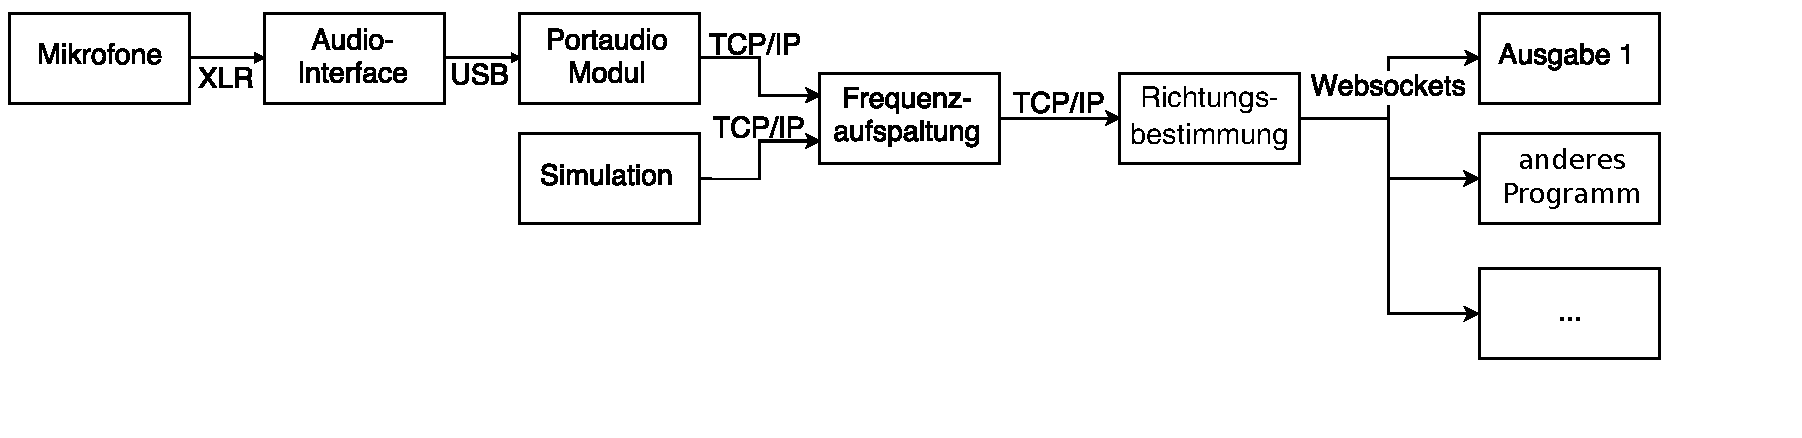
\includegraphics[width=\linewidth]{img/flowchart}
	\caption{Der modulare Aufbau unseres Konzeptes} 
	\label{fig:flowchart}
\end{figure}
Unser Konzept sieht vier Module vor, welche über TCP/IP und Websockets verbunden sind. Dies sind Standards, über die über ein Computernetzwerk Daten ausgetauscht werden können \cite{tcp} \cite{websockets}. Diese beiden Protokolle sind sehr zuverlässig und und lange erprobt. Außerdem garantieren diese, dass alle Daten in der Reihenfolge, in der sie losgeschickt werden, ankommen. Die Verwendung von Netzwerkprotokollen hat den Vorteil, dass die Module nicht unbedingt auf demselben Computer ausgeführt werden müssen und so der Rechenaufwand bei Bedarf auf mehrere Computer verteilt werden kann.\\
\subsection{Modul 1: Eingabe/Aufnahme}
Das erste Modul in dieser Kette stellt die Rohdaten für die weitere Verarbeitung bereit. Diese  können entweder von einer Gruppe real existierender Mikrofone stammen oder, im Falle der Simulation, die Signale einer Gruppe simulierter Mikrofone, die simulierte Schallquellen aufnehmen, sein.

\subsection{Modul 2: Signal aufteilen}
Im zweiten Modul der Kette wird das Signal, welches aus dem ersten Modul stammt, in die einzelnen im Signal enthaltenen Wellen aufgeteilt, also von einer zeitaufgelösten Form in ein frequenzaufgelöstes Signal umgewandelt. Nach diesem Schritt liegt also für jede Frequenz eine Amplitude und eine Phase vor. In diesem Modul werden außerdem Frequenzen, welche nicht oder nur sehr leise in dem Eingangssignal vorkommen, herausgefiltert, um das Rauschen und den benötigten Rechenaufwand in den nächsten Modulen zu verringern.\\

\subsection{Modul 3: Ortung}
Das nächste Modul empfängt die Daten des vorherigen Moduls und errechnet zunächst für jede Frequenz aus den transformierten Daten den Gangunterschied zwischen den Signalen der Mikrofone. Aus diesen werden dann die möglichen Ursprungspunkte der Sinusschwingung ermittelt.

\subsection{Modul 4: Ausgabe}
Das letzte Modul in der Signalkette ist die Ausgabe. Sie bekommt die fertig gruppierten Schallquellen über eine Websocket-Verbindung und bereitet sie für den Nutzer auf. Dieses Modul kann auf die jeweilige Anwendung angepasst werden und es können mehrere Output-Module mit dem gleichen Ortungs-Modul verbunden werden.